\chapter{序論}


\section{研究背景}
\subsection*{量子コンピューターの課題}
近年、量子コンピューターが話題に上がることが多くなってきた。
量子コンピューターは超並列計算機とも呼ばれ、因数分解、最適化計算に優れる。同時に話題になっているAI(ディープラーニング)はビックデータなどを対象に最適化問題に応用されるため、量子コンピューターとの相性が良いこともその一因であると考えられる。既に商用化された量子コンピュータもあるが、まだまだ課題は多い。
量子コンピューターの情報担体である量子ビットには量子性を破壊せず制御できる仕組みが必要だが、現在それができる仕組みは少なく、実用化には様々な制約がある。
その中で最も有力だと言われているものが「超伝導回路」による量子ビットである。
超伝導回路ではジョセフソン接合を用いて量子もつれ状態を実現しているが、
情報の保存時間であるコヒーレンス時間が現在数十マイク秒程度であり、
極低温下でしか動作しないなどの課題も多い。
北野研究室では、その課題解決に向けて高温超伝導体の固有ジョセフソン接合
(IJJ:Intrinsic Josephson Junction)を用いた超伝導量子ビットの実現を目指している。

\subsection*{ジョセフソン接合}
二つの超伝導体が弱く結合した接合をジョセフソン接合と呼ぶ。
超伝導状態では、2つの電子が引力相互作用によりクーパー対を形成し、
巨視的な数のクーパー対の状態が重ね合わされて、超伝導基底状態が記述されることになる。
この基底状態を記述する関数を巨視的波動関数と呼ぶ。
ジョセフソン接合では2つの(巨視的波動関数の位相が異る)
超伝導体間に薄い絶縁体を挟むなどして弱く結合させることにより、
接合間にトンネル電流が流れる現象(ジョセフソン効果)が見られる。

Fig1.1にジョセフソン接合の
模式図を示す。
\vspace{5 mm}

\begin{figure}[h]
  \begin{center}
    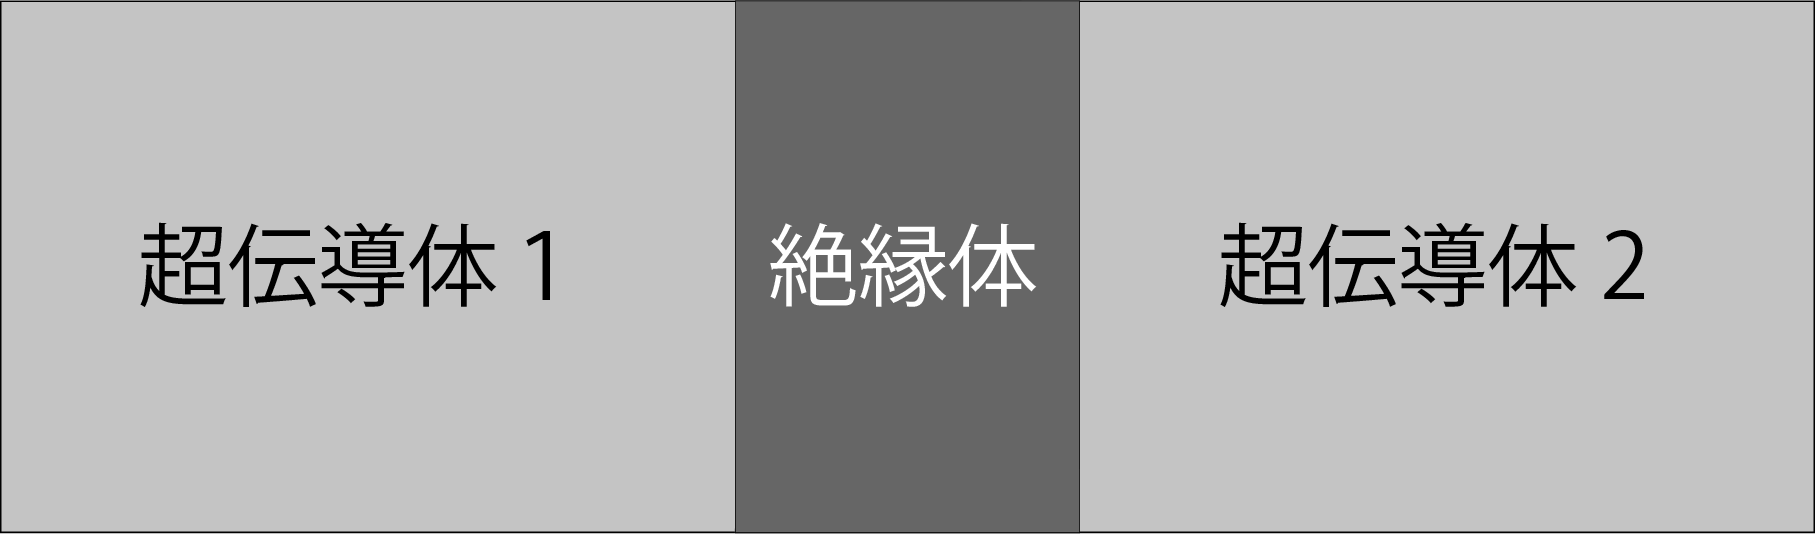
\includegraphics[width=5cm]{./image/JJ.png}
    \caption{ジョセフソン接合の模式図}
    \label{fig:JJ}
  \end{center}
\end{figure}
2つの超伝導体の巨視的波動関数の位相差を$ \Delta \theta $とすると、そこに流れる超伝導電流$I$は以下のように記述できる。

\begin{eqnarray}
   I = I_c \sin{\Delta \theta }
\end{eqnarray}

\subsection*{固有ジョセフソン接合}
超伝導物質の中には、その物質内部に絶縁体と超伝導体が非常に薄い層状に重なっている構造をもつ層状超伝導体が存在する。
そのような構造は結晶構造に固有なジョセフソン接合と見なすことができる。これを固有ジョセフソン接合と呼ぶ。
以下にその例として、銅酸化物高温超伝導体Bi$_2$Sr$_2$CaCu$_2$O$_y$(以下、Bi2212と略記)の結晶構造をFig1.2示す\cite{びすます}。
\vspace{10 mm}

\begin{figure}[h]
  \begin{center}
    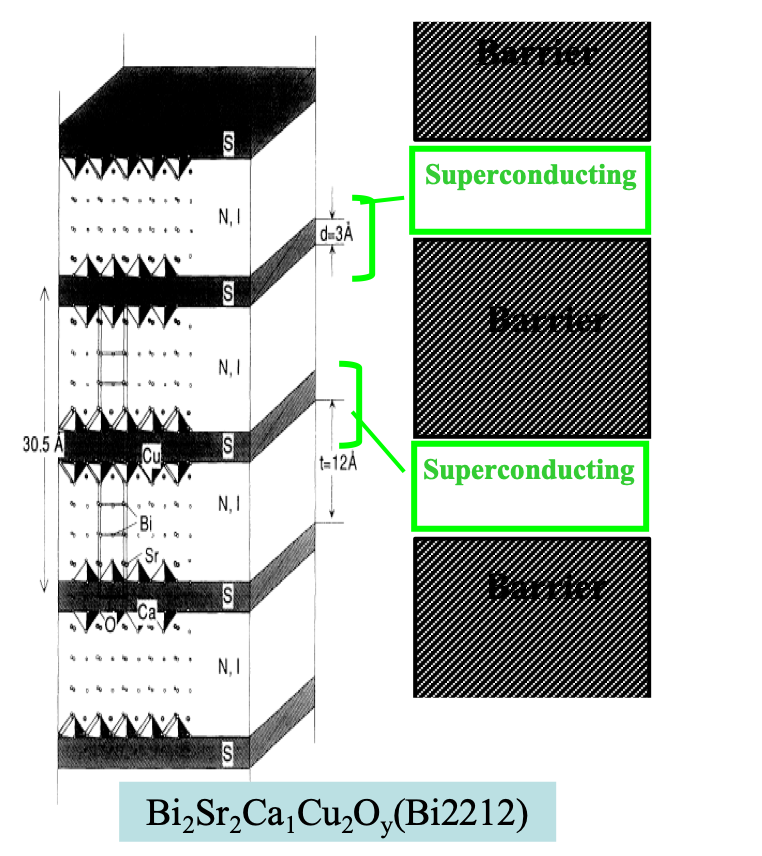
\includegraphics[width=5cm]{./image/IJJ.png}
    \caption{Bi2212の層状構造}
    \label{fig:Cavity}
  \end{center}
\end{figure}

北野研究室では、Bi2212系固有ジョセフソン接合の研究を行っている。一例として、2015年度の修士論文研究(高橋優作氏)\cite{たかはし}では、Bi2212単結晶から作製された固有ジョセフソン接合素子に41.5GHzのマイクロ波を照射した際電圧状態へスイッチする電流の確率分布に2重ピーク構造が観測された。このことから巨視的量子トンネル状態への移行と離散化量子準位の形成が示唆された。
このほかにも、北野研の過去の研究では40〜60GHz程度のマイクロ波照射で、同様の離散化順位の形成が観測された。

しかし固有ジョセフソン接合素子は、人工的に作製したジョセフソン素子とは異なり、実際に測定するまで離散化準位の形成が観測できるマイクロ波周波数がわからない。
% 素子の作成方法を工夫して、エネルギー順位を調整することは大変困難であるため、
これは人工的ジョセフソン接合における回路定数が、固有ジョセフソン接合では
物質定数に支配され、素子設計の自由度が制限されるためである。
したがって、
素子作成後にどの程度のエネルギー準位を有しているか調べるための方法が必要である。
今回は空洞共振器を用いてその準位を調べることを目指す。

\section{予備知識}
\subsection*{マイクロ波空洞共振器}
マイクロ波とは周波数が数GHzから数十GHzほどの領域にある電磁波で、波長が電波より短く、遠赤外線より長い領域にある電磁波である。

一般に、高周波電流の流れている導体の周囲には電流を囲む円周方向に磁界$H$、あるいは磁束密度$B =μH$($μ$は媒質の透磁率)の磁束が生じる。
これは電磁気学におけるアンペールの法則として知られている現象である。
この磁束は、電流の周波数によって変化するため、ファラデーの電磁誘導則より、磁束に垂直な方向に電界E、あるいは電束密度$D =εE$(ここで$ε$は媒質の誘電率)で与えられる時間的に変化する電束が生じる。
このような電束の変化はそこに電流が流れていると同等に考えてよいため、再び新たな磁界が発生する。このようにして、伝搬していく波を電磁波と呼んでいる。電磁波は真空中でも伝搬する。

ある形状の管の中に音波を伝播させると特定の周波数で大きな音がなる現象は共振現象と呼ばれ、
管楽器など身近なところにも応用されている馴染みの深い現象であるが、
マイクロ波でも同様な現象が起こる。
一般に完全導体で閉じられた中空の箱の中でマイクロ波を照射すると、
電磁場エネルギーが箱の中に蓄えられ、特定の周波数で電磁界振幅が増大する共振現象が起きる。
この中空の箱のことを空洞共振器と呼び、共振時の周波数を共振周波数と呼ぶ。
一般に空洞共振器の共振周波数は、閉じられた空間を表す境界条件の下、マクスウェル方程式の固有値解として与えられ、
空洞の形や大きさに依存して複数の固有値を持つことが知られている。

境界のない自由空間での電磁波は、進行方向に対して垂直な向きに電磁界が発生するため、
TEMモード(TEM:$Transverse Electro-Magnetic Wave$,TEM波とも)と呼ばれる。
一方、空洞共振器では、内部構造と固有値によって定まる定在波が
特定の方向にできるような固有モードを持つ。
簡単のため、導波管(完全導体の中空の筒)内の伝播モードを考える。
導体壁で囲まれた導波管中を電磁波が伝搬していく場合、
導体面における境界条件(電界は導体面に垂直、磁界は平行)から、TEM波の伝播は不可能である。
進行方向を$z$とすると境界条件を満たして$z$方向に進行することができるモードとして次の2つが存在する。
電界の進行方向成分$E_z $はゼロであるが、
磁界の進行方向成分$H_z$は存在する電磁波のことをTE波($Tranceverse Electric Wave$)、
逆に$H_z$はゼロであるが、$E_z$は存在する電磁波のことを
TM波($Tranceverse Magnetic Wave$)と呼び、導波管内ではこの2つのモードが伝播する。

空洞共振器では導波管とは異なり、進行方向という概念は存在しない。
そのため、本研究では直方体食うフォウの3辺の長さ $x,y,z$ のうち、
$y<x<z$となるように長さを設定し、$z$を進行方向成分とみてモードの同定を行った。
方形空洞共振器の共振周波数は以下の式 (1.2)で決まる。
ここで、$a,b,l$は図1.3に示す直方空洞の各辺長、$m,n,p$は$a,b,l$の各方向成分の腹の数を示す整数である。
方形空洞共振器の場合、$a,b,l$と$m,n,p$が同一の$TE$モードと$TM$モードは互いに縮退している。

\vspace{10 mm}

\begin{figure}[h]
  \begin{center}
    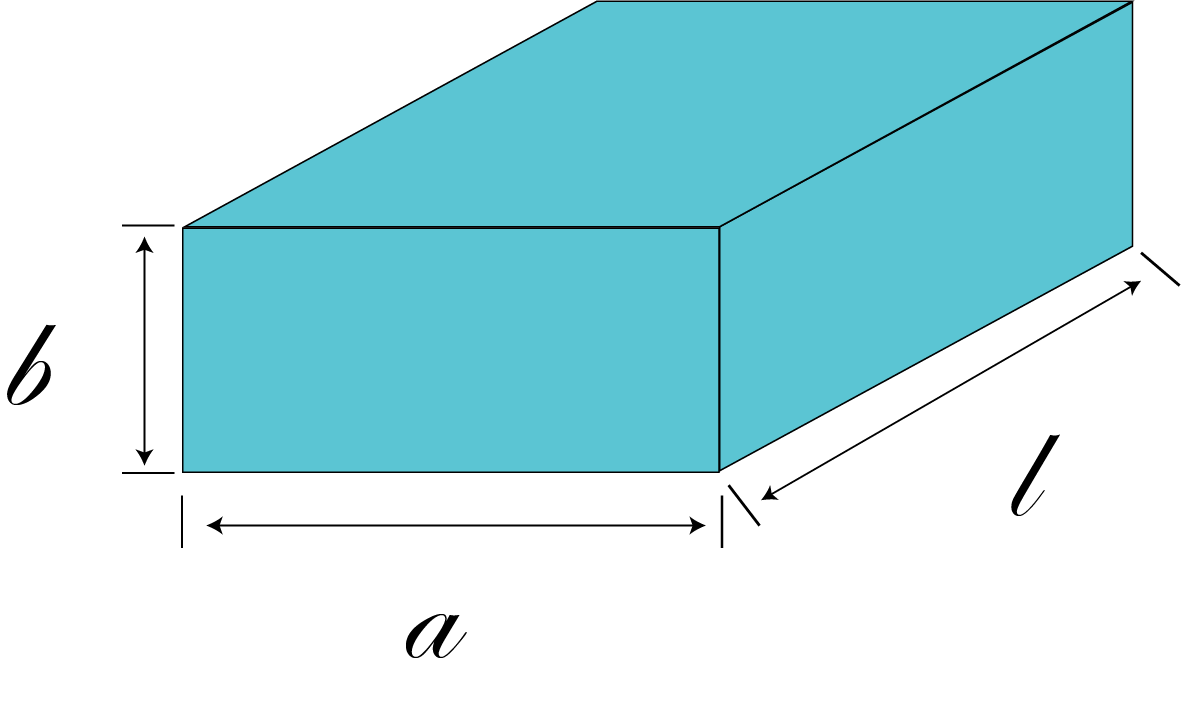
\includegraphics[width=8cm]{./image/空洞共振器.png}
    \caption{方形空洞共振器}
    \label{fig:Cavity}
  \end{center}
\end{figure}

\begin{eqnarray}
    \frac{1}{\lambda} = (\frac{m}{2a})^2 + (\frac{n}{2b})^2 + (\frac{p}{2l})^2
\end{eqnarray}

\subsection*{空洞量子電磁力学実験}
Fig1.4のように共振器内に単一原子を置き、
内部の原子と電場の間の電気双極子結合を利用して、
単一量子システムを制御する物理をc-QED($cavity - Quantum ElectroDynamics$)と呼ぶ。
超伝導量子ビットは人工的に作られた原子系とみなせるので、
光子→マイクロ波(共振器内の1モード)、
原子→人工原子(超伝導量子ビット)に
置き換えたシステムが調べられている。
人工的ジョセフソン接合を用いたc-QED実験は、マイクロ波共振器が平面回路で作製されるためcurcuit-QEDとも呼ばれる。
